%
% Copyright (c) 2020 Antonio Coín Castro
%
% This work is licensed under a
% Creative Commons Attribution-ShareAlike 4.0 International License.
%
% You should have received a copy of the license along with this
% work. If not, see <http://creativecommons.org/licenses/by-sa/4.0/>.

In this chapter we will introduce the basic terminology needed to understand the theory that will subsequently be developed. We will present ordinary differential equations and their solutions in a rigorous manner, as well as some concepts intimately related to them, such as integral curves and initial value problems, and analyze how these equations fit into the general theory of differentiable functions. At the same time, we will set the notation that will be used throughout the exposition. The main reference for this chapter is \cite{petrovski1966ordinary}.

\section{Ordinary differential equations}

By an \textit{ordinary differential equation of order $n$} we mean a relation of the form
\begin{equation}
\label{eq:ode}
F(x, y, y', \dots, y^{(n)}) = 0,
\end{equation}
where $F$ is a real-valued function of $n+1$ real variables, $x$ is an independent variable, $y=y(x)$ is an unknown function and $y', \dots, y^{(n)}$ are the first $n$ derivatives of this function with respect to $x$. When the value of $n$ is understood or simply not relevant, we will refer to \eqref{eq:ode} only as an ordinary differential equation (\acrshort{ode}), with the word \textit{ordinary} meaning that the unknown function depends solely on one independent variable. A central concept in our study will be that of a solution of such a differential equation, which is rigorously defined below.

\begin{definition}
  \label{def:solution}
  A \textit{solution} of the differential equation \eqref{eq:ode} is a function $\phi: I \to \R$, where $I=(a,b)$, $-\infty \leq a < b \leq \infty$ is some open interval of the real line, satisfying the following conditions:

  \begin{enumerate}
    \item The function $\phi$ has derivatives up to order $n$;
    \item The identity $F(x, \phi(x), \phi'(x), \dots, \phi^{(n)}(x)) = 0$ holds for all $x \in I$.
  \end{enumerate}
  The process of finding solutions of a differential equation is also known as \textit{integrating} the equation.
\end{definition}

From now on, unless otherwise stated we will restrict ourselves to \textit{first order} ODEs, which take the general form
\begin{equation}\label{eq:fode}
  F(x,y,y') = 0,
\end{equation}
and thus their solutions are differentiable functions of $x$ that reduce the equation to an identity when substituted for $y$. Furthermore, we will initially consider differential equations in \textit{explicit} form, that is,
\begin{equation}
  \label{eq:fode-explicit}
  y' = f(x, y),
\end{equation}
and we will assume that the function $f(x,y)$ is defined on some domain (open and connected subset) $G$ of the $(x,y)$-plane.

\begin{remark}
  Sometimes we will find it more useful to use Leibniz's notation and express the above equation as
  \begin{equation*}
    \der = f(x,y).
  \end{equation*}

\end{remark}

\section{Geometric interpretation of ODEs}

Continuing our description of differential equations, we shall now present a natural interpretation of equations such as \eqref{eq:fode-explicit} and a way to visualize them in the plane. To begin with, suppose that we draw a short line segment through every point $(x,y)$ of $G$ with slope equal to $f(x,y)$, obtaining a set of directions in $G$ that is called the \textit{direction field} of equation \eqref{eq:fode-explicit}. In other words, we transform our (known) function $f$ in a vector field on its domain. At this point we can restate the problem of solving \eqref{eq:fode-explicit} from a geometric perspective:
\begin{quotation}
  \itshape \noindent
  Find all differentiable curves $y=\phi(x)$ in $G$ whose tangents have directions belonging to the direction field of \eqref{eq:fode-explicit}.
\end{quotation}
To see how this is equivalent to solving \eqref{eq:fode-explicit}, one need only recall that the slope of the tangent of a (differentiable) curve at any point coincides with its derivative at that point, and then look at Definition \ref{def:solution}. However, this formulation of the problem has two noticeable caveats from a geometric point of view:

\begin{enumerate}[1.]
  \item By considering only \textit{graphs} over the $x$-axis we are excluding curves that are intersected more than once by vertical lines.
  \item The imposition that the slope of the direction field generated in $G$ be given by $f$ automatically excludes directions parallel to the $y$-axis, because $f$ would need to be infinite at those points.
\end{enumerate}

We are interested in looking at solutions of differential equations in a more general setting. This is why, based on the previous reformulation, we will develop a broader concept of solution with a strong geometrical meaning, one that will address both difficulties outlined above. In the first place, we allow general curves in parametric form, that is, $x=\lambda(t)$, $y=\mu(t)$, $-\infty \leq \alpha < t < \beta \leq \infty$. This solves the first problem. To overcome the second limitation, in addition to equation \eqref{eq:fode-explicit} we consider the associated differential equation
\begin{equation}
  \tag{\ref*{eq:fode-explicit}'}
  \label{eq:fode-explicit1}
  \frac{dx}{dy} = f_1(x,y),
\end{equation}
where
\begin{equation*}
  f_1(x,y) = \frac{1}{f(x,y)}.
\end{equation*}
The rationale behind this decision is to allow the function $f$ to become infinite at some points (representing a vertical slope), and shift our perspective from the $x$-axis to the $y$-axis at those points. In this way, at points where both $f$ and $f_1$ are defined we can use either \eqref{eq:fode-explicit} or \eqref{eq:fode-explicit1} to construct the direction field, but we use \eqref{eq:fode-explicit1} at points where $f$ becomes infinite\footnote{At each point of $G$, at least one of $f$ or $f_1$ is always defined, for $f=0$ if and only if $f_1$ is infinite, and $f_1=0$ if and only if $f$ is infinite.}.

We are now ready to define our new, more general concept of solution, which will necessarily be related not only to the original equation, but also to the newly defined associated equation. We will restrict ourselves to the class of \textit{smooth} \textit{regular} curves, that is, continuously differentiable curves with non-vanishing derivative everywhere. From now on, all curves will implicitly be assumed to belong to this class.

\begin{definition}\label{def:integral-curves}
  An \textit{integral curve} of equations \eqref{eq:fode-explicit} and \eqref{eq:fode-explicit1} is a smooth regular curve whose tangent at each point has a direction specified by the direction field of said equations.
\end{definition}

Given that equations \eqref{eq:fode-explicit} and \eqref{eq:fode-explicit1} are closely related, sometimes we will use the singular form to encompass both of them as a single equation. As we are looking at curves in parametric form, to obtain an explicit formula in this case we may first apply the chain rule,
\begin{equation*}
  \frac{dy}{dt} = \der \frac{dx}{dt},
\end{equation*}
and then we solve for $dy/dx$, getting
\begin{equation}
  \label{eq:fode-mn}
  \der = \frac{dy/dt}{dx/dt} = \frac{M(x, y)}{N(x, y)}.
\end{equation}
If the chosen curve does indeed satisfy the equation, then $f = M/N$ will hold. For simplicity we will seldom write down explicitly the associated equation,
\begin{equation}
  \tag{\ref*{eq:fode-mn}'}
  \frac{dx}{dy} = \frac{N(x,y)}{M(x,y)} = f_1(x,y),
\end{equation}
but we shall sometimes write \eqref{eq:fode-mn} as
\begin{equation*}
  M\,dx - N\, dy = 0,
\end{equation*}
to stress the symmetry in $x$ and $y$. This equation specifies a direction field at every point where both $M$ and $N$ are defined and at least one of them is nonzero.

Even though we are allowing general curves in parametric form, they are not (the graph of) a true solution of our equation unless we restrict them to some interval in which they can be expressed as a graph. We can think of the family of all solutions to equation \eqref{eq:fode-explicit} as a subset of the family of integral curves of \eqref{eq:fode-explicit} and \eqref{eq:fode-explicit1}, restricted to a suitable interval if need be. An example visualization of direction fields and integral curves is shown in Figure \ref{fig:integral-curves-ex}.

\begin{figure}[h!]
  \centering
  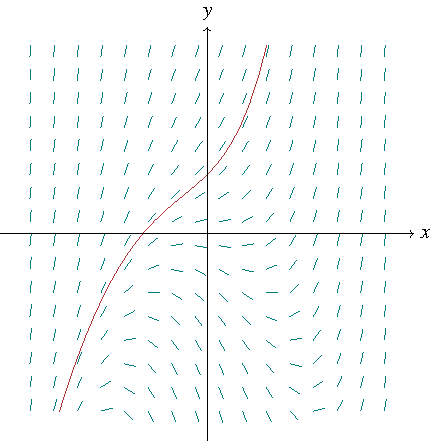
\includegraphics[width=.5\textwidth]{integral-curves-1}
  \caption{Direction field of the equation $y'=x^2+y$ near the origin and a particular integral curve.}
  \label{fig:integral-curves-ex}
\end{figure}

The requirement that integral curves be regular guarantees that we can always shrink their domain so that they become a graph, and hence a solution to our differential equation. The following result delves into that question.

\begin{prop}
  Every point in a smooth regular curve belongs to an arc which is a smooth graph.
\end{prop}

\begin{proof}
  Let $x=\lambda(t)$, $y=\mu(t)$, $\alpha < t < \beta$ be a smooth regular curve, and pick $t_0 \in (\alpha, \beta)$. The regularity of the curve guarantees that either $\lambda'(t_0)$ or $\mu'(t_0)$ is nonzero, so suppose without loss of generality that $\lambda'(t_0) \neq 0$. Since $\lambda'(t_0)$ is continuous by assumption, there exists an $\epsilon > 0$ such that $\lambda'(t)\neq 0$ for $t \in (t_0 - \epsilon, t_0 + \epsilon)$, and then the equation $x=\lambda(t)$ has a unique smooth solution in $t$ by virtue of the \textit{inverse function theorem} (see \cite[372]{apostol1974analysis}). Then, by eventually shrinking $\epsilon$ we may write $t=\psi(x)$, $\lambda(t_0 - \epsilon) < x < \lambda(t_0 + \epsilon)$. Substituting in $y=\mu(t)$ yields $y=\mu(\psi(x)) = \phi(x)$, $\lambda(t_0 - \epsilon) < x < \lambda(t_0 + \epsilon)$, which is the equation of a smooth graph.
\end{proof}

\begin{remark} The conditions on integral curves in Definition \ref{def:integral-curves} imply that our solutions are also smooth, that is, continuously differentiable.
\end{remark}

We can illustrate the previous definitions and properties with a simple example.

\begin{example}
  Consider the equation
  \begin{equation*}
    \der = \frac{y}{x},
  \end{equation*}
  which we can also write as
  \begin{equation*}
    x\,dy = y\,dx.
  \end{equation*}
  Solving it by elementary methods gives the family of solutions
  \begin{equation*}
    y =kx, \quad x \in \R - \{0\}, \ k \in \R.
  \end{equation*}
  On the other hand, this equation defines a direction field in the whole plane minus the origin. To find its integral curves we consider the associated equation $dx/dy = x/y$ in the subset
  \begin{equation*}
    \{(0, y): y \in \R - \{0\}\}
  \end{equation*}
  of the plane. Combining both equations we can see that the set of all integral curves is given by the relation
  \begin{equation*}
    ax+by=0, \quad (x,y), (a, b) \in \R^2 - \{(0,0)\}.
  \end{equation*}
  The direction field is shown schematically in Figure \ref{fig:integral-curves-ex-2}. Notice that we have found two integral curves for this equation that are not the graph of any solution, namely the two vertical rays emanating from the origin.
  \begin{figure}[h!]
    \centering
    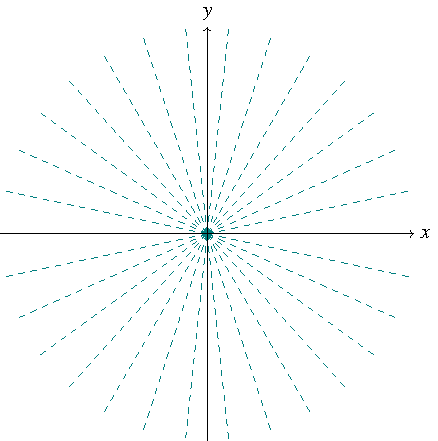
\includegraphics[width=.5\textwidth]{integral-curves-2}
    \caption{Direction field of the equation $x\,dy = y\, dx$ near the origin.}
    \label{fig:integral-curves-ex-2}
  \end{figure}
\end{example}

As a closing remark, we note that we could have ignored the directions parallel to the $y$-axis altogether, and we still would have ended up with a well defined, reasonable concept of integral curve. This is in fact what V. Arnold does in \cite{cooke1992ordinary}. However, taking these conflicting points into account will allow us to better study and understand \textit{singularities} of the function $f$, allowing for a more general perspective and broadening the scope of this work.

\section{Existence and uniqueness of solutions}

So far we have been talking about solutions of a differential equation without stopping to think even if such solutions exist in the first place. Could we come up with an equation which has no solutions at all? To answer this question, remember that any possible solution is assumed to be smooth, and thus its derivative verifies the \textit{intermediate value theorem}\footnote{\label{fn:darboux} A similar argument for non-smooth solutions may be given using \textit{Darboux's theorem} \cite[112]{apostol1974analysis}, which states that the derivative of any differentiable function that takes two different values on an interval must take every value in between.}. But this derivative must be equal to $f$, so it suffices to choose a function that does not have the intermediate value property. For example, if we consider the famous Dirichlet function
\begin{equation*}
  g(x) = \begin{cases}
    1  & \text{if } x \in \mathbb{Q},\\
    0  &\text{elsewhere},
\end{cases}
\end{equation*}
then the equation $y'=f(x, y) = g(x)$ has no solutions.

From this example we can speculate that the lack of continuity of $f(x,y)$ is the key property that makes the equation unsolvable. This is indeed the case, as it turns out that existence of solutions is always guaranteed if we impose that $f$ be continuous.

\begin{theorem}[Peano's existence theorem] Let $f(x,y)$ be a continuous function on a domain $G\subset \R^2$. Then the differential equation
  \begin{equation*}
    y' = f(x,y)
  \end{equation*}
has at least one solution in $G$. Moreover, if $f$ is continuous on a neighbourhood of a point $(x_0, y_0) \in G$, then there exists a solution $\phi$ defined on a neighbourhood of $x_0$ satisfying $\phi(x_0)=y_0$.
\end{theorem}

\begin{proof}
  See \cite{peano1890demonstration} for Peano's original 1890 proof, which uses a method known as successive approximations. Shorter proofs have been proposed since, many using topological arguments such as fixed points theorems (see for example \cite[14]{hale1980ode}).
\end{proof}

\begin{remark} If we assume continuity of the function $f$, then the smoothness of any solution comes as a consequence and not as a hypothesis, since $\phi'(x) = f(x, \phi(x))$. In fact, the level of regularity of the function $f$ translates in a similar manner to the solutions: if $f$ has continuous derivatives up to order $m$, then any solution to $y'=f(x,y)$ has continuous derivatives up to order $m+1$.

\end{remark}

The concept of a solution passing through a predefined point is not incidental to our study, but it plays a major role in much of the subsequent theory, which is why it merits its own denomination. A differential equation $y'=f(x,y)$ coupled with an \textit{initial condition} $y(x_0)=y_0$ is called an \textit{initial value problem}, often abbreviated as \acrshort{ivp}. With this new definition in mind, Peano's theorem states that every initial value problem defined by a continuous function has at least one solution, or more generally, that there is at least one integral curve of the equation passing through the selected point.

Together with the question of existence comes inevitably the issue of uniqueness. Peano's theorem guarantees that under mild conditions a solution to an initial value problem always exists, but it does not say anything about it being unique. It is not hard to think of an example in which uniqueness of solution is violated. For instance, it is immediate to verify that the IVP

\begin{equation*}
  \begin{cases} y' = 3y^{2/3},\\
    y(0)=0

  \end{cases}
\end{equation*}
has two valid solutions: $y=0$ and $y=x^3$. Thus some kind of additional condition is needed to ensure that one and only one integral curve passes through a given point, as the following theorem asserts.

\begin{theorem}[Picard-Lindelöf] \label{th:picard}
  Let $G \subset \R^2$ be a domain in the plane, and suppose $f:G \to \R$ is a continuous function that locally satisfies a Lipschitz condition in the second variable, that is, for every $p \in G$ there exists a neighbourhood $U_p$ of $p$ in $G$ and a constant $L>0$ such that
\begin{equation*}
  \abs{f(x, y_2) - f(x, y_1)} \leq L\abs{y_2 - y_1}
\end{equation*}
whenever $(x,y_1),(x,y_2) \in U$. Then for every point $(x_0, y_0) \in G$ the initial value problem
  \begin{equation}
  \begin{cases} y' = f(x, y) & \text{in } G,\\
    y(x_0)= y_0
  \end{cases}
\end{equation}
has exactly one solution.
\end{theorem}

\begin{proof}
  A proof in modern terms can be found in \cite[36]{teschl2012ordinary}. The idea is to construct a sequence of approximate solutions, the so-called method of \textit{Picard iterations}, and then leverage the Lipschitz condition to apply the \textit{contraction principle}\footnote{Also known as \textit{Banach fixed point theorem}, after Polish mathematician Stefan Banach who first proved it in 1922 \cite{banach1922operations}.}.
\end{proof}

\begin{remark}
  The Lipschitz condition on Theorem \ref{th:picard} can be relaxed to a condition on the partial derivative. The theorem remains true, via a direct application of the \textit{mean value theorem}, if $\partial f / \partial y$ is locally bounded, which in turn holds if said partial derivative is continuous on $G$. This condition is often easier to check.
\end{remark}

Bringing back the geometric interpretation of differential equations, it is straightforward to see that at points where there is uniqueness of solutions two integral curves can never be tangent to each other (they cannot cross either by definition). However, it is precisely the points in which uniqueness fails that interest us, and we will study them in depth in the following chapter.
